\begin{frame}
  \frametitle{Biquadratic Adaptivity}
  \begin{center}
	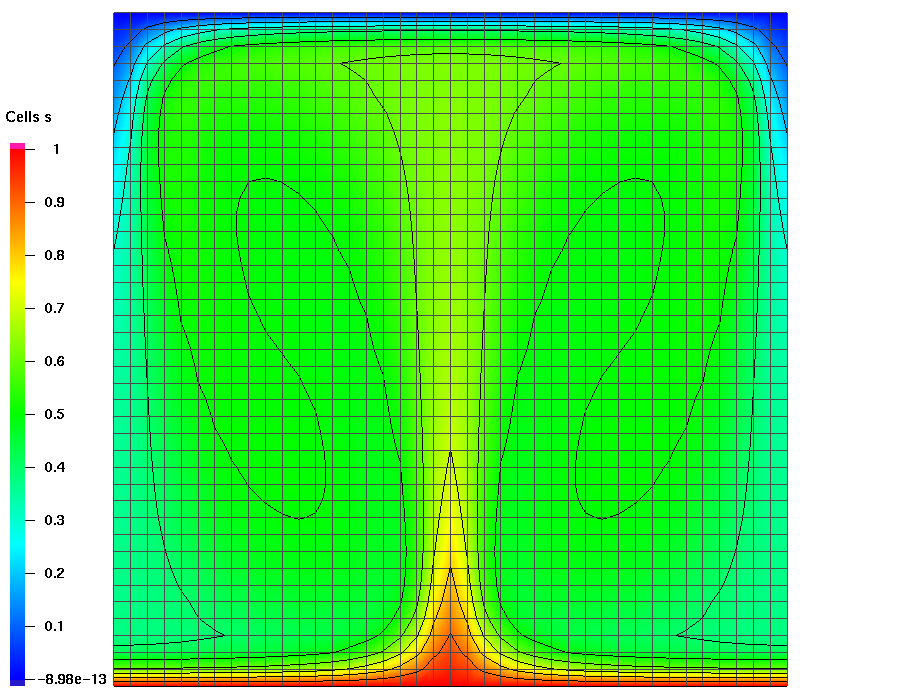
\includegraphics[width=.8\textwidth]{figures/biquad_amr_0000}    
  \end{center}
\end{frame}
  
\begin{frame}
  \frametitle{Biquadratic Adaptivity}
  \begin{center}
	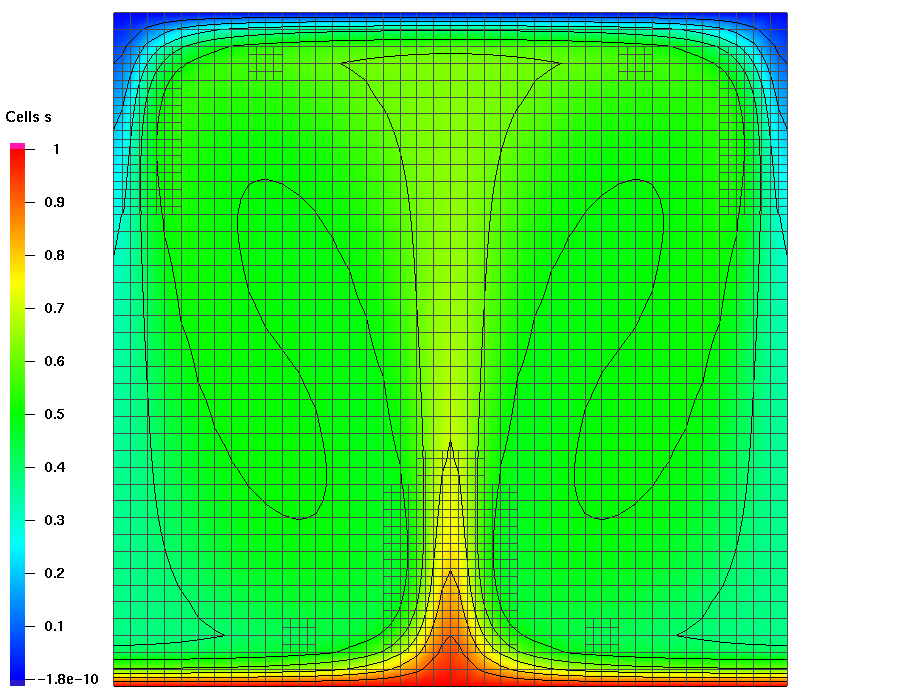
\includegraphics[width=.8\textwidth]{figures/biquad_amr_0001}    
  \end{center}
\end{frame}

  \begin{frame}
  \frametitle{Biquadratic Adaptivity}
  \begin{center}
	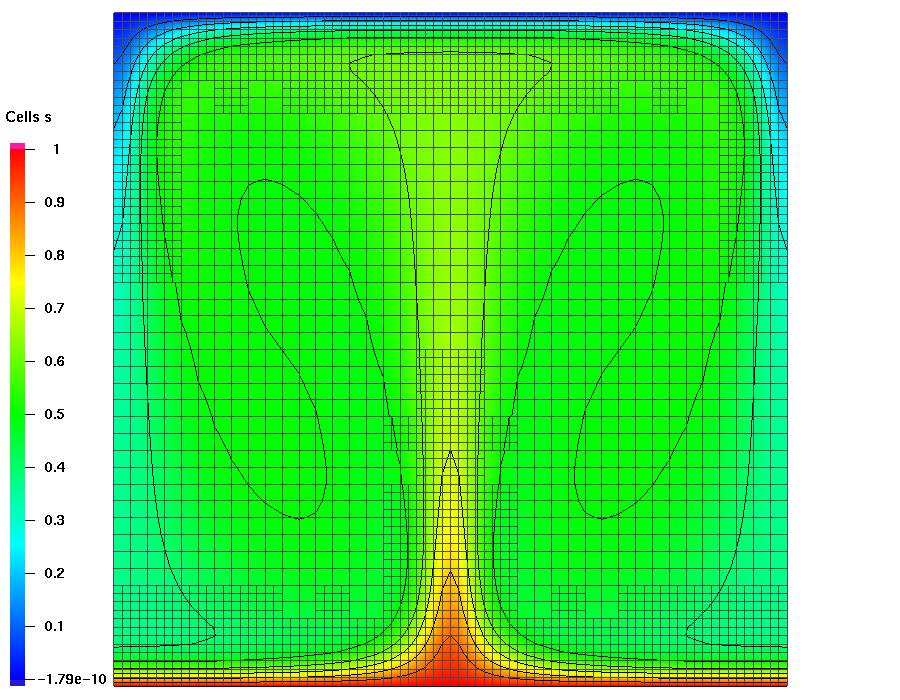
\includegraphics[width=.8\textwidth]{figures/biquad_amr_0002}    
  \end{center}
\end{frame}
\begin{frame}
  \frametitle{Biquadratic Adaptivity}
  \begin{center}
	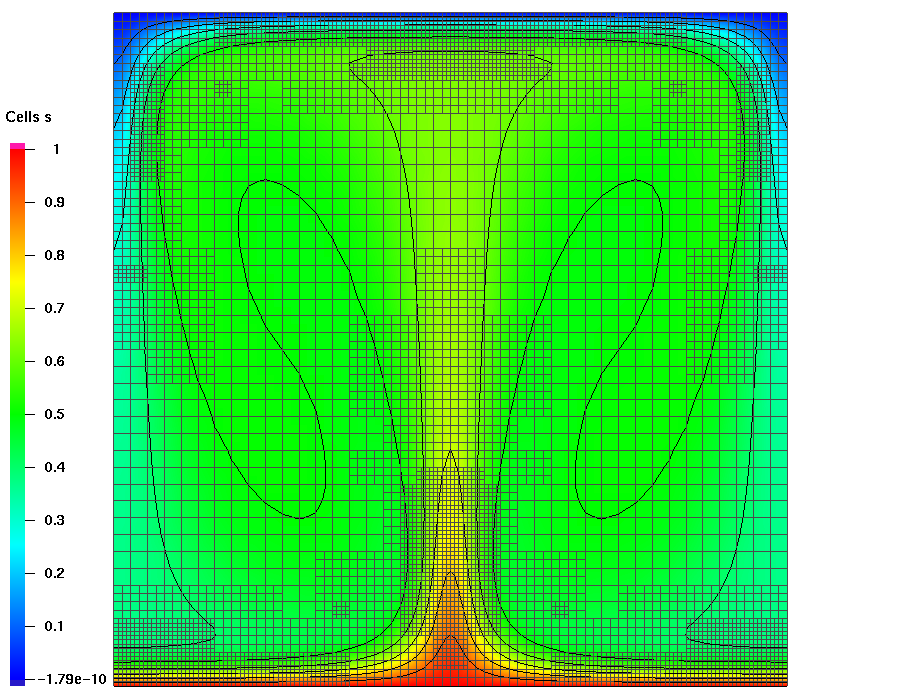
\includegraphics[width=.8\textwidth]{figures/biquad_amr_0003}    
  \end{center}
\end{frame}
\begin{frame}
  \frametitle{Biquadratic Adaptivity}
  \begin{center}
	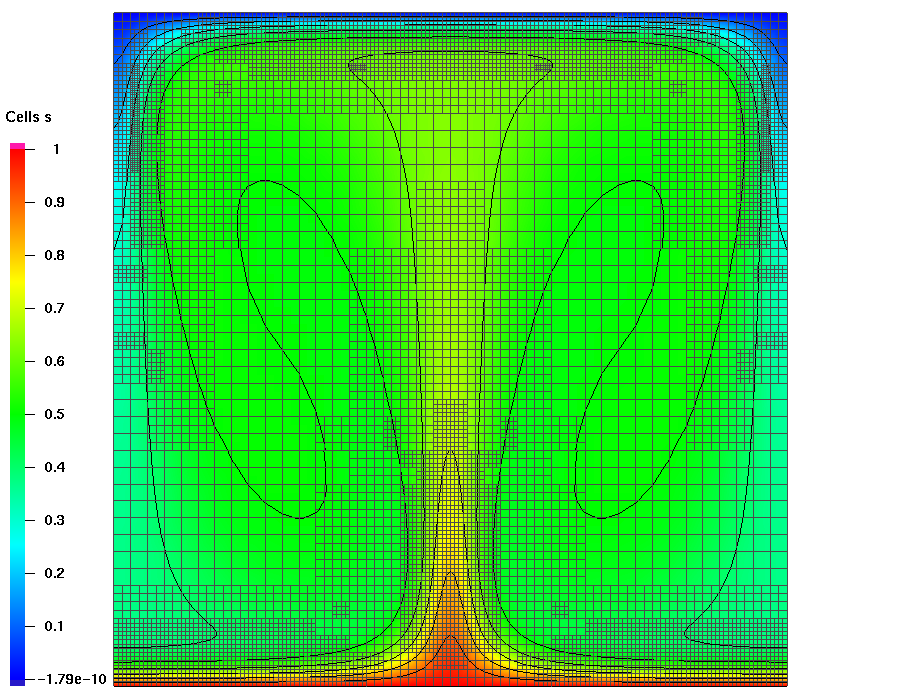
\includegraphics[width=.8\textwidth]{figures/biquad_amr_0004}    
  \end{center}
\end{frame}
\begin{frame}
  \frametitle{Biquadratic Adaptivity}
  \begin{center}
	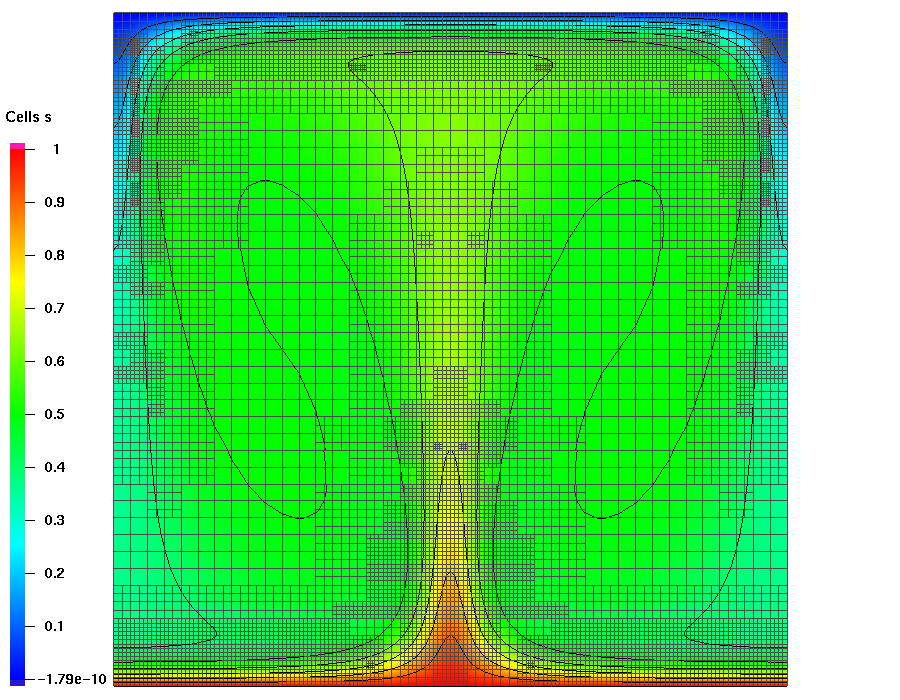
\includegraphics[width=.8\textwidth]{figures/biquad_amr_0005}    
  \end{center}
\end{frame}
\begin{frame}
  \frametitle{Biquadratic Adaptivity}
  \begin{center}
	\includegraphics[width=.9\textwidth]{figures/biquad_adapt_vs_unif_thermal}    
  \end{center}
\end{frame}
\begin{frame}
  \frametitle{Biquadratic Adaptivity}
  \begin{center}
	\includegraphics[width=.9\textwidth]{figures/biquad_adapt_vs_unif_solute}    
  \end{center}
\end{frame}





